\documentclass[tikz, border=1mm]{standalone}
\usepackage{tikz} 
\usetikzlibrary{arrows.meta}
\usepackage{pgfplots}

\begin{document}

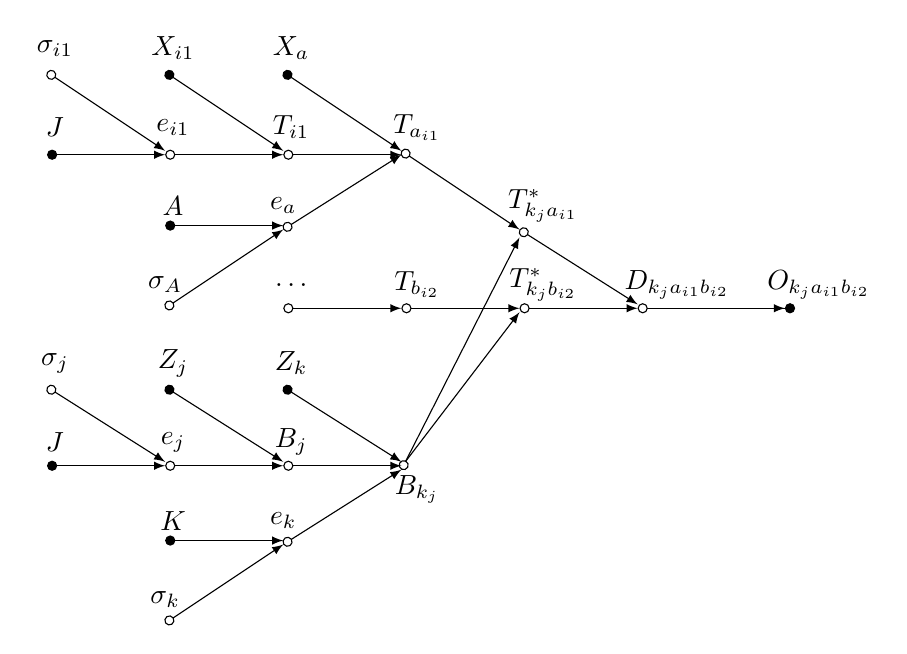
\begin{tikzpicture}

    % outcome
    \node at (3.8,1.3) {$O_{{k_{j}a_{i1}b_{i2}}}$};

    % discriminal difference
    \node at (2,1.3) {$D_{{k_{j}a_{i1}b_{i2}}}$};
    \draw[{Circle[open]}-{latex}{Circle}](1.5,1) to (3.5,1); 
    
    % "perceived" discriminal process for sub-unit
    \node at (0.3,2.3) {$T^{*}_{k_{j}a_{i1}}$};
    \draw[{Circle[open]}-{latex}](0,2) to (1.5,1.05); 

    % "true" discriminal process for sub-unit
    \node at (-1.3,3.3) {$T_{a_{i1}}$};
    \draw[{Circle[open]}-{latex}](-1.5,3) to (0,2);

    % predictors for sub-unit
    \node at (-2.9,4.3) {$X_{a}$};
    \draw[{Circle}-{latex}](-3,4) to (-1.5,3);

    % "true" discriminal process of unit
    \node at (-2.9,3.3) {$T_{i1}$};
    \draw[{Circle[open]}-{latex}](-3,2.95) to (-1.5,2.95);

    % predictors for units
    \node at (-4.4,4.3) {$X_{i1}$};
    \draw[{Circle}-{latex}](-4.5,4) to (-3,3);

    % units trait error
    \node at (-4.4,3.3) {$e_{i1}$};
    \draw[{Circle[open]}-{latex}](-4.5,2.95) to (-3,2.95);

    % units error variance
    \node at (-5.9,4.3) {$\sigma_{i1}$};
    \draw[{Circle[open]}-{latex}](-6,4) to (-4.5,3);

    % units population size
    \node at (-5.9,3.3) {$J$};
    \draw[{Circle}-{latex}](-6,2.95) to (-4.5,2.95);

    % sub-units error
    \node at (-3,2.3) {$e_{a}$};
    \draw[{Circle[open]}-{latex}](-3,2) to (-1.5,2.95);

    % sub-units population size
    \node at (-4.4,2.3) {$A$};
    \draw[{Circle}-{latex}](-4.5,2.05) to (-3,2.05);

    % sub-units error variance
    \node at (-4.5,1.3) {$\sigma_{A}$};
    \draw[{Circle[open]}-{latex}](-4.5,1) to (-3,2);




    % "perceived" discriminal process for stimulus b_{i2}
    \node at (0.3,1.3) {$T^{*}_{k_{j}b_{i2}}$};
    \draw[{Circle[open]}-{latex}](0,1) to (1.5,1);
    
    % "true" discriminal process for stimulus b_{i2}
    \node at (-1.3,1.3) {$T_{b_{i2}}$};
    \draw[{Circle[open]}-{latex}](-1.5,1) to (0,1); 

    % extras for stimulus b_{i2}
    \node at (-2.9,1.3) {$\dots$};
    \draw[{Circle[open]}-{latex}](-3,1) to (-1.5,1); 





    % repeated judges' bias k_{j}
    \node at (-1.3,-1.3) {$B_{k_{j}}$};
    \draw[{Circle[open]}-{latex}](-1.5,-1.05) to (0,1.90);
    \draw[-{latex}](-1.45,-0.95) to (0,0.95);

    % predictors for repeated judges' bias
    \node at (-2.9,0.3) {$Z_{k}$};
    \draw[{Circle}-{latex}](-3,0) to (-1.5,-0.95);

    % judges' bias
    \node at (-2.9,-0.7) {$B_{j}$};
    \draw[{Circle[open]}-{latex}](-3,-1) to (-1.5,-1);

    % predictors for judges' bias
    \node at (-4.4,0.3) {$Z_{j}$};
    \draw[{Circle}-{latex}](-4.5,0) to (-3,-0.95);

    % judges' bias error
    \node at (-4.4,-0.7) {$e_{j}$};
    \draw[{Circle[open]}-{latex}](-4.5,-1) to (-3,-1);

    % judges' bias error variance
    \node at (-5.9,0.3) {$\sigma_{j}$};
    \draw[{Circle[open]}-{latex}](-6,0) to (-4.5,-0.95);

    % judges' population size
    \node at (-5.9,-0.7) {$J$};
    \draw[{Circle}-{latex}](-6,-1) to (-4.5,-1);

    % repeated judges' bias error
    \node at (-3,-1.7) {$e_{k}$};
    \draw[{Circle[open]}-{latex}](-3,-2) to (-1.5,-1.05);

    % repeated comparisosn population size
    \node at (-4.4,-1.7) {$K$};
    \draw[{Circle}-{latex}](-4.5,-1.95) to (-3,-1.95);

    % judges' bias error variance
    \node at (-4.5,-2.7) {$\sigma_{k}$};
    \draw[{Circle[open]}-{latex}](-4.5,-3) to (-3,-2);
    
\end{tikzpicture}

\end{document}
